\documentclass{article}
\usepackage[top=2.54cm, bottom=2.54cm, left=2.54cm, right=2.54cm]{geometry}
\usepackage{graphicx}
\setlength{\parskip}{12pt}
\setlength{\parindent}{0pt}
\begin{document}

\begin{center} Huilin Tong\\
ID:1261574
\end{center}

{\bf Discussion}\\

\begin{enumerate}

\item The computer get the right answer for Problem 1.
\item The population reached a stable constant in the end: $n_0= 571$ for 0-1 years age group, $n_1= 342$ for 1-2 years age group, $n_2= 274$ for 2-3 years age group, $n_3= 182$ for 3-4 years age group, $n_{total}=1371$ for total population.

\item The population achieved exponential growth in Problem 3.
The growth rate is $1.022$ for each age group and the total population.
\item Yes, they should be the same.
\item Yes, population should grow faster.
\item (Extra Credit)

What are the stable ratios $n_1/n_0$, $n_2/n_1$ and $n_3/n_2$ that the age-group populations will satisfy? 

The stable ratios equals to the survival rate. $n_1/n_0=p_0$, $n_2/n_1=p_1$ and $n_3/n_2=p_2$
\begin{center}
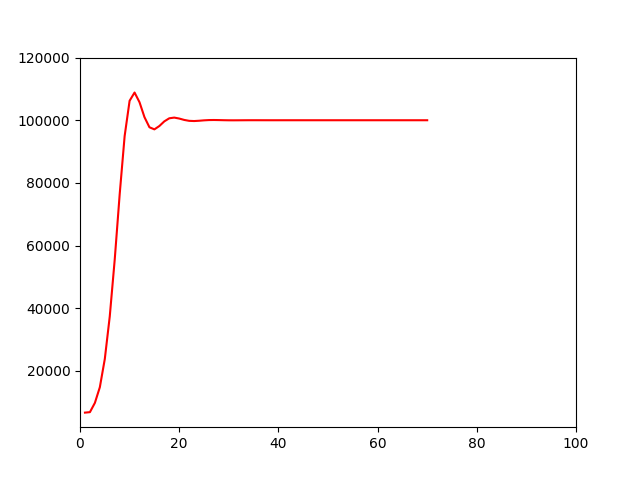
\includegraphics[scale=0.7]{graph3.png}

Fig.1 Total population when k=100000
\end{center}

Suppose $k=100000$. Set the birth rate keep decreasing with the increase of total population. When the total population reach the capacity, then birth rate also remains unchanged. Such birth rate should satisfy the requirement to keep population at a stable size.
\begin{center}
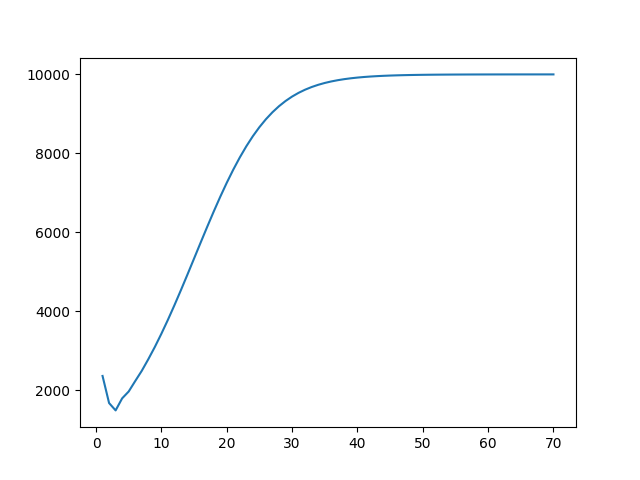
\includegraphics[scale=0.7]{graph.png}

Fig.2 Total population when k=10000
\end{center}

If set $k=10000$, and keep birth rate change at a slow speed. The total population will change like fig.2.

\begin{center}
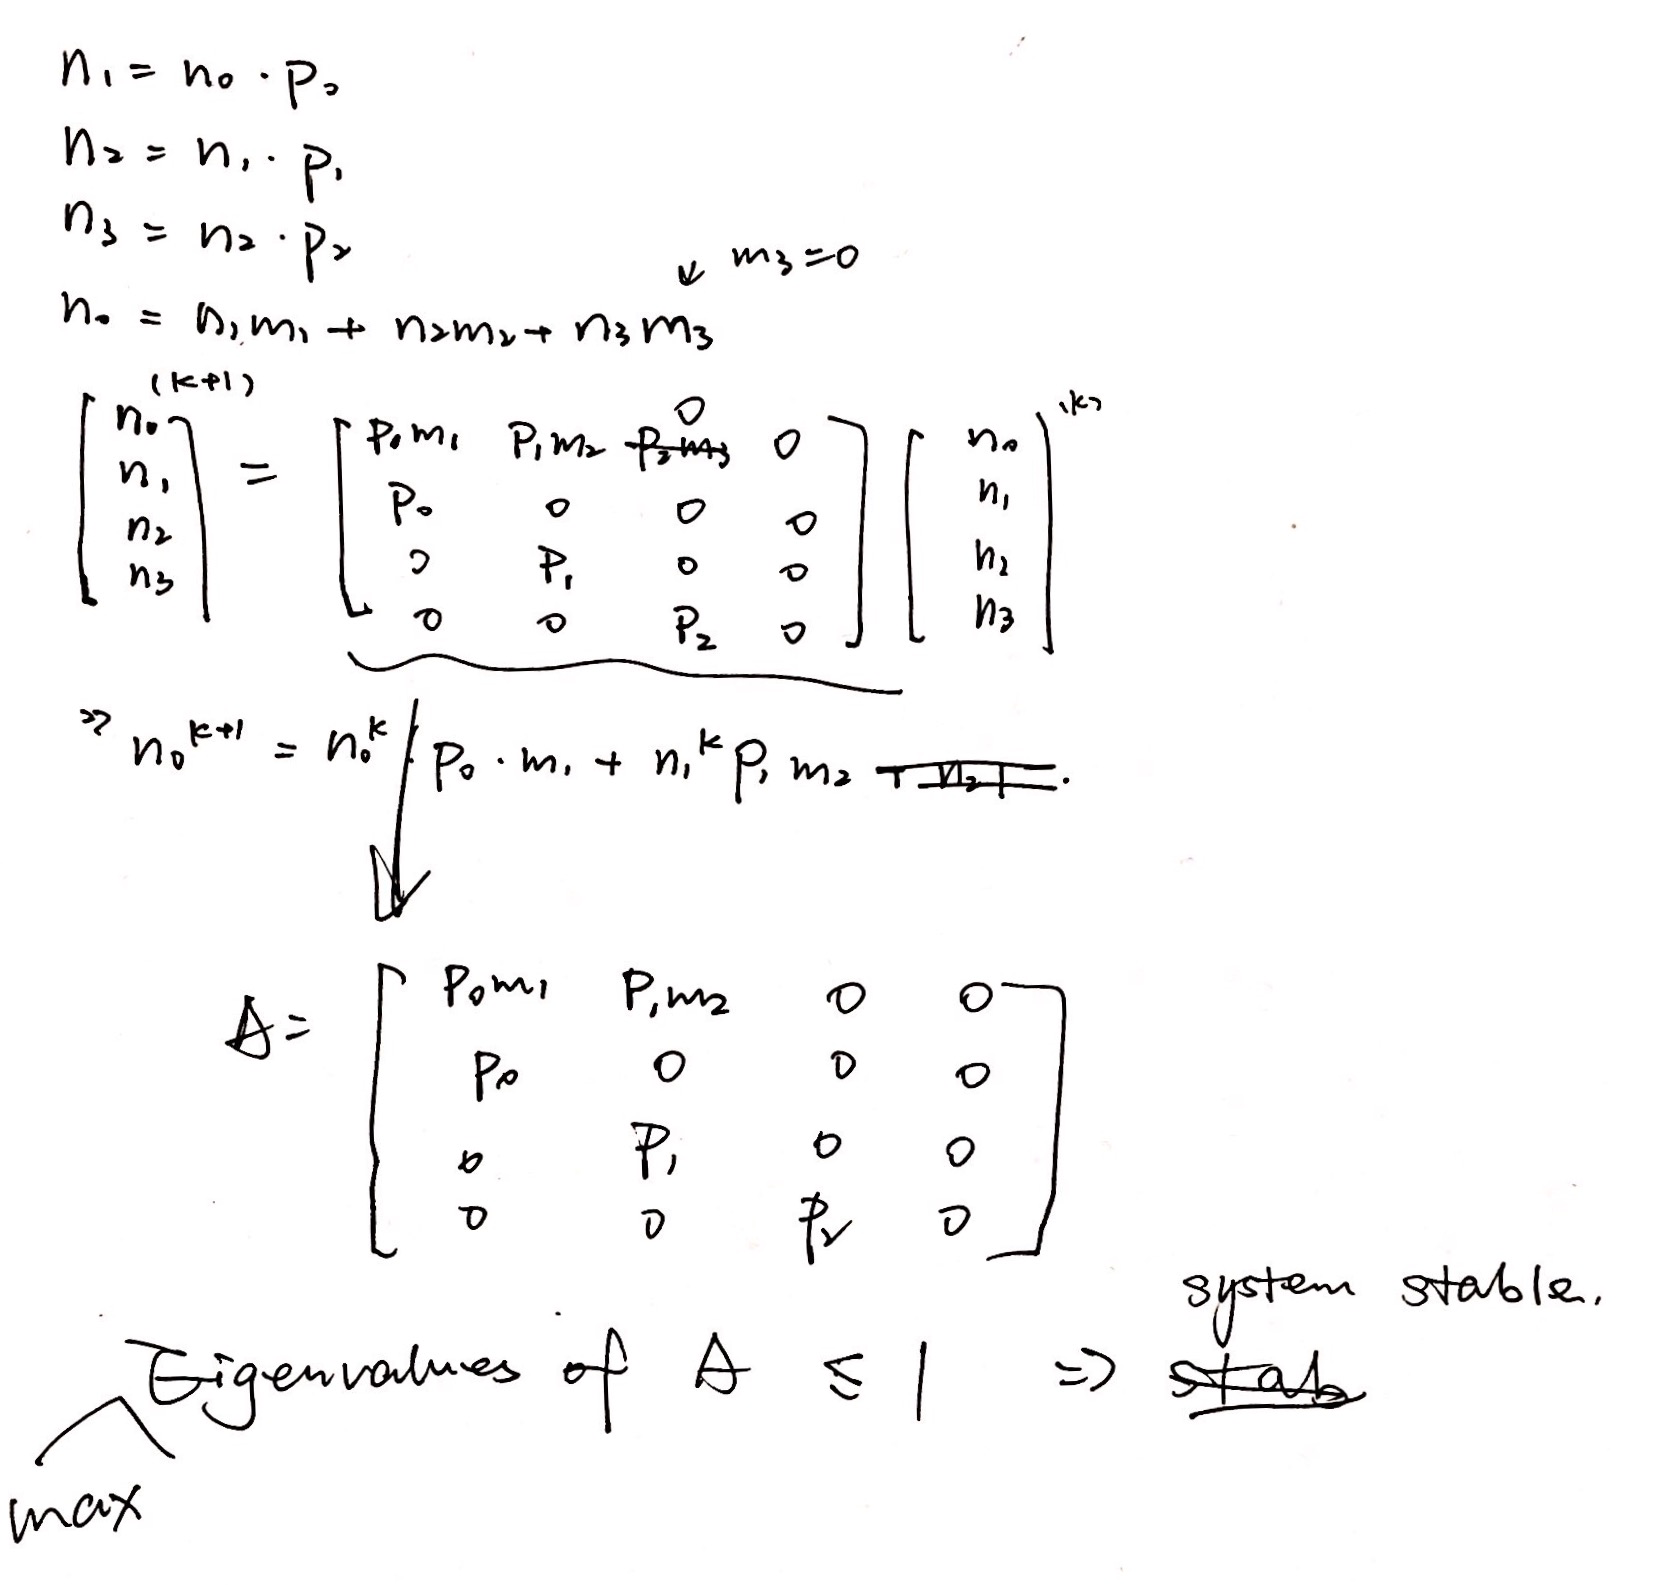
\includegraphics[scale=0.2]{hw1_pic.png}
\end{center}
The four eigenvalues of $A$ is 
\begin{center}
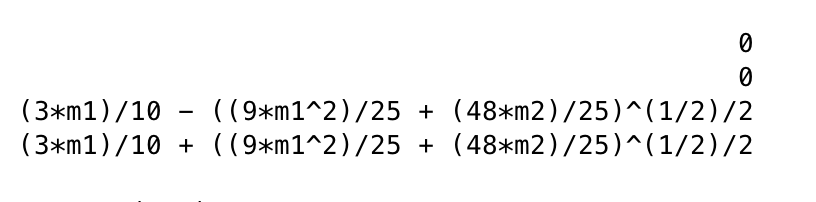
\includegraphics[scale=0.65]{eig.png}
\end{center}

So the sable birth rate should meet the requirement as $\frac{3*m_1}{10} + \frac{1}{2}\sqrt[2]{\frac{9*m_1^2}{25} + \frac{48*m_2}{25}}\le 1$
\end{enumerate}
\end{document}